\svnid{$Id$}
\appendix
\chapter{Appendix}
\section{\texorpdfstring{Monte Carlo Estimation of $\pi$}{Monte Carlo Estimation of Pi}}
\begin{figure}[ht]
 \centering
 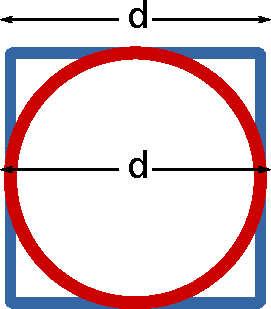
\includegraphics[width=7cm, trim=0cm 0cm 0cm 0.3cm]{./appendix/data/monte-carlo-pi.pdf}
 % monte-carlo-pi.pdf: 130x148 pixel, 72dpi, 4.59x5.22 cm, bb=0 0 130 148
 \caption[Circle circumscribed by a square]{{\bf Circle circumscribed by a square.} A Circle of diameter $d$ inside a square of side $d$.
 \label{fig:circle-square}}
\end{figure}
\noindent Using the example shown in Figure \ref{fig:circle-square}:
\begin{itemize}
 \item The area of the square is $d^2$.
 \item The area of the circumscribed circle is $\pi\times\left(\frac{d}{2}\right)^2 = \frac{\pi}{4}\times d^2$.
 \item The ratio of the two is therefore $\frac{\frac{\pi}{4}\times d^2}{d^2} = \frac{\pi}{4}$.
\end{itemize}
Pi can be estimated by calculating the ratio of randomly distributed points that fall within the circle to those that fall within the square.

\section{Adaptive step sizes and numerical instability}
An adaptive step size routine was required for the ordinary differential equation algorithm to prevent numerical instability issues from arising and producing bogus results. At points during the simulation, a number of parameters can take on very small values, or are changing rapidly and a fixed step size algorithm can cause problems here by assuming that the value stays small, or stays constant during the length of the fixed step. The result of these assumptions is numerical instability whereby the erroneous values of these parameters affects other parameters in the simulation. The most obvious and disastrous effect is of concentrations in the simulation going negative.

To prevent this issue an adaptive step size was implemented whereby if the parameters are changing slowly the step size can be large, but this is adaptively decreased (and conversely increased) when parameters are changing more quickly. In the absence of an adaptive step size routine, the fixed step size would have to be set small enough to solve the rapidly changing regions correctly, but would then be unnecessarily small in the slowly changing regions.

\section{\texorpdfstring{Affinity of \cbbthree{} for Oxygen}{Affinity of cbb3 for Oxygen}}
A large amount of data was gathered during the course of this work of oxygen reduction which could be used for analysis of the affinity of \cbbthree{} for oxygen. Simple observation of these datasets which can be seen in Chapter \ref{chap:oxygenreduction} shows that \cbbthree{} must have a high affinity for oxygen by virtue of the fact that oxygen reduction continues linearly all the way down to almost zero oxygen. A lower oxygen affinity would show a marked slowing of the reduction rate as the concentration of oxygen decreased. A simple was of visualising the change in rate during oxygen reduction is to plot the instantaneous rate against the concentration of oxygen.

A more appropriate way to visualise the rates is to use a Lineweaver-Burk (double reciprocal) plot. This allows the $V_{max}$ and $K_m$ to be calculated from a regression line through the data. The x-axis intercept is equal to $-\frac{1}{K_m}$, and the y-axis intercept is equal to $\frac{1}{V_{max}}$. A Lineweaver-Burk plot for a representative oxygen reduction dataset is shown in Figure \ref{fig:o2lb}.
\begin{figure}[ht]
 \centering
 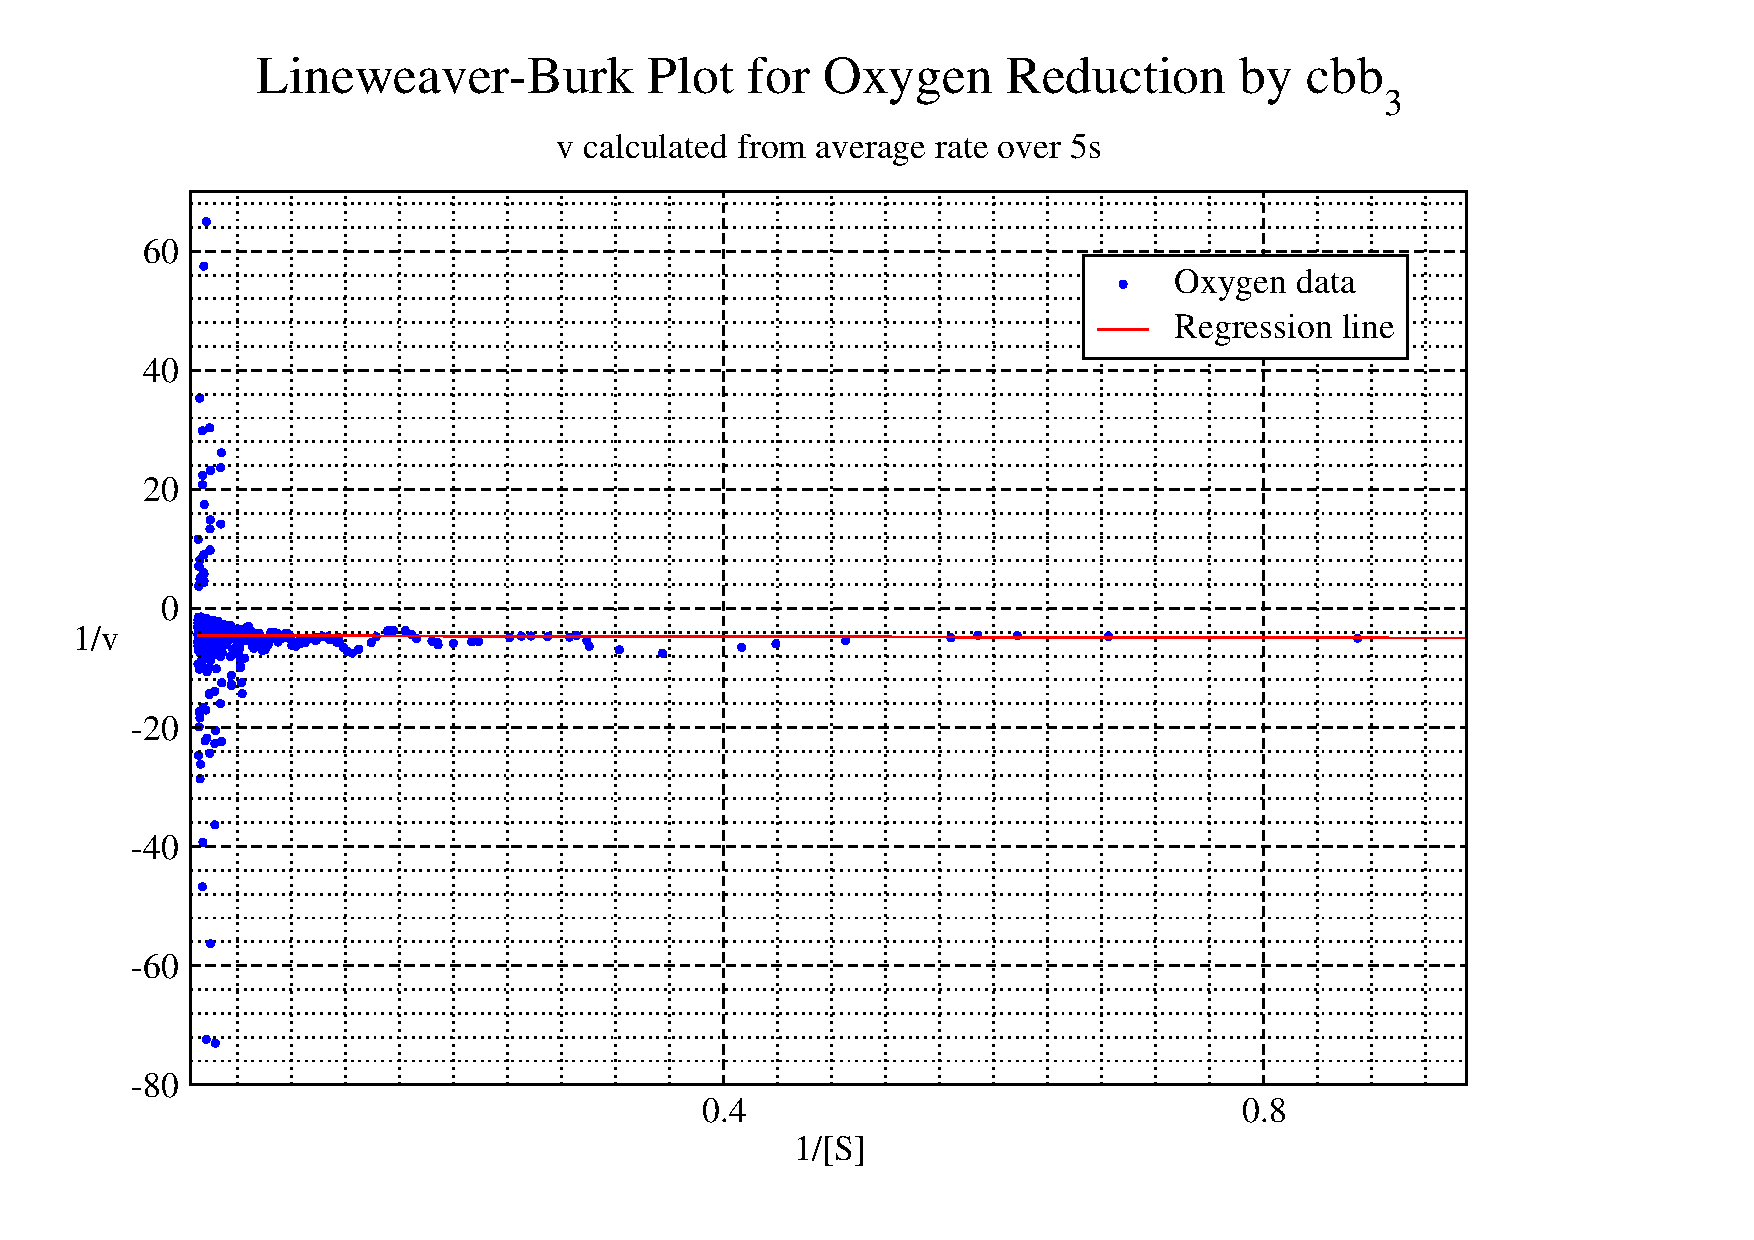
\includegraphics[width=14cm, trim=1cm 1cm 4cm 0.5cm, clip=true]{./appendix/data/lbplot.pdf}
 % o2sim.eps: 0x0 pixel, 300dpi, 0.00x0.00 cm, bb=0 0 794 595
 \caption[{Lineweaver-Burk Plot for Oxygen Reduction in \textit{Neisseria meningitidis}.}]{{\bf Lineweaver-Burk Plot for Oxygen Reduction in \textit{Neisseria meningitidis}}. V was calculated as a 5 second rolling average rate to try and smooth out some of the data. The rates are largely negative as oxygen was being removed from the system. The regression line shown is a simple linear regression through all datapoints.
 \label{fig:o2lb}}
\end{figure}

Unfortunately the combination of particularly noisy data generated by the oxygen electron, and the limited sampling rate (of $1 s^-1$) mean that the degree of affinity could not be explored further. The essentially flat regression line through the Lineweaver-Burk plot here would imply a completely linear reduction rate and extremely high affinity of \cbbthree{} for oxygen.


\begin{eqnarray}
\frac{d[O_2]}{dt} & = & \beta\left(1-\frac{[O_2]}{K_O}\right) - k_{1}[C_a][O_2] \nonumber \\
\frac{d[NO]}{dt} & = & m_{1}[NO_2^-][A_a] - l_1[NO][B_a] - k_5[C_a][NO] + k_6[C_X] - \gamma[NO] \nonumber \\
\frac{d[NO_2^-]}{dt} & = & - m_{1}[NO_2^-][A_a] \nonumber \\
\frac{d[Q_a]}{dt} & = & g([Q] - [Q_a]) - l_3[Q_a]([B] - [B_a]) - f[Q_a]([X]-[X_a])\ \nonumber \\
\frac{d[X_a]}{dt} & = & -k_3([C] - [C_a] - [C_X])[X_a] - m_3([A] - [A_a])[X_a] + f[Q_a]([X]-[X_a]) \nonumber \\
\frac{d[A_a]}{dt} & = & m_3([A] - [A_a])[X_a] - m_{1}[NO_2^-][A_a] \nonumber \\
\frac{d[B_a]}{dt} & = & l_3[Q_a]([B] - [B_a]) - l_1[NO][B_a] \nonumber \\
\frac{d[C_a]}{dt} & = & k_3([C] - [C_a] - [C_X])[X_a] - k_{1}[C_a][O_2] - k_{5}[C_a][NO] \nonumber \\
\frac{d[C_X]}{dt} & = & k_5[C_a][NO] - k_6 [C_X] \nonumber \\
\frac{d[A]}{dt} & = & \left(R\left(1 - \frac{[O_2] + k_{10}[NO]}{[O_2] + k_{10}[NO] + k_{11}}\right) - S\left(1 - \frac{[NO]}{[NO] + k_{13}}\right)\right) - k_8[A] \nonumber \\
\frac{d[B]}{dt} & = & T \left(\frac{[NO]}{[NO] + k_{15}}\right) - k_{16}[B]
\end{eqnarray}

\begin{table}[ht]
\begin{center}
\begin{tabular}{lcc}
\toprule
\textbf{Symbol} & & \textbf{Description}\\
\midrule
$O_2$ & & Oxygen concentration\\
$NO$ & & Nitric oxide concentration\\
$NO_2^-$ & & Nitrite concentration\\
$X_a$ & & Reduced cytochrome concentration\\
$A_a$& & Reduced AniA\\
$B_a$& & Reduced NorB\\
$C_a$& & Reduced \cbbthree{}\\
$C_X$& & Reversibly inhibited \cbbthree{}\\
$Q_a$& & Reduced Quinones\\
\bottomrule
\end{tabular}
\caption{Model Variables
\label{vs}}
\end{center}
\end{table}



\begin{table}[ht]
\begin{center}
\begin{tabular}{l c}
\toprule
\textbf{Symbol} & \textbf{Description}\\
\midrule
$k_1$ & Rate constant for O$_{\textrm{2}}$ reduction by reduced \cbbthree{}\\
$k_3$ & Rate constant for \cbbthree{} reduction by cytochrome pool\\
$l_1$ & Rate constant for NO reduction by reduced NorB\\
$l_3$ & Rate constant for NorB reduction by quinone pool\\
$m_1$ & Rate constant for NO$_{\textrm{2}}^{\textrm{-}}$ reduction by reduced AniA\\
$m_3$ & Rate constant for AniA reduction by cytochrome pool\\
$k_5$ & Rate constant for \cbbthree{} inhibition by NO\\
$k_6$ & Rate constant for recovery of NO inhibited \cbbthree{}\\
$\beta$ & Rate constant for passive diffusion in of O$_{\textrm{2}}$\\
$K_O$ & Saturation O$_{\textrm{2}}$ level\\
$g$ & Rate of electrons in from NADH\\
$f$ & Rate constant for reduction of cytochromes by quinones\\
$\gamma$ & Spontaneous loss of NO\\
$Q$ & Concentration of quinones\\
$X$ & Concentration of cytochromes\\
$A$ & Concentration of AniA\\
$B$ & Concentration of NorB\\
$C$ & Concentration of \cbbthree{}\\
\bottomrule
\end{tabular}
\caption{Model Parameters
\label{ps}}
\end{center}
\end{table}